

\section{Ruppert-Polyak-Juditsky Averaging}

\textbf{Goal:}
$$
\mathrm{min} \  f(\theta) = \frac{1}{n}\sum_{i=1}^{n}f(\theta, z_i)
$$
where $f(\theta)$ is a strongly convex function. \\

\textbf{Method:}\\
Similar with previous, we use the following update:
$$
\theta_{k+1} = \theta_k - \gamma_kg(\theta_k,z_k)
$$
with $g(\theta_k,z_k)$ be the noisy gradient. Furthermore, we then set step size to be
$$
\gamma_k = \frac{c}{k^\alpha}
$$
Theoretically $\alpha$ can be any number in $(\frac{1}{2}, 1)$.\\

%Although in general we don't assume smoothness, in this method we assume $f$ is  $L$ smooth.


The final estimator we use is the average:
$$
\bar{\theta_k} = \frac{\theta_1 + ... + \theta_k}{k}
$$


\textbf{Result:}\\

\begin{assumption}
	$f(\theta)$ is $m$-strongly convex function and $L$-smooth. Furthermore, the noisy gradient has the following realization:
$$
g(\theta_k, z_k) = \nabla f(\theta_k) + \xi_k
$$
Where
$$
\mathbb{E}(\xi_k|\xi_1,...,\xi_{k-1}) = 0
$$
$$
\mathbb{E}(\Vert \xi_k\Vert^2|\xi_1,...,\xi_{k-1}) \leq c
$$
\end{assumption}

\begin{theorem}
Under assumptions above, if we take step size to be $\gamma_k = \frac{c}{k^\alpha}$ with $\alpha$ in $(\frac{1}{2}, 1)$, then:
$$
\sqrt{k}(\bar{\theta_k} - \theta^*) \xrightarrow{k \rightarrow \infty} \mathbf{N}(0,V)
$$
where
$$
V = (\nabla^2f(\theta^*))^{-1}S(\nabla^2f(\theta^*))^{-1}
$$
with $S = cov(g(\theta^*,z))$.
\end{theorem}

%Then three professors derive the distribution:\\
Here we actually choose step size larger than the original SGD paper \cite{RM51}.

%remarkable distributional result(not easy in optimization)


Notice that in Polyak and Juditsky's original paper \cite{PJ92}, the assumption: $\mathbb{E}(\Vert \xi_k\Vert^2|\xi_1,...,\xi_{k-1}) \leq c$ can be further loosed by the tail behavior of $\xi_k$'s distribution.\\

\textbf{Remarks:}

1. If $f$ is the negative log likelihood of parameter $\theta^*$, then both $S$ and Hessian $\nabla^2f(\theta^*)$ are the Fisher information $I$. Then we will have:
$$
\sqrt{k}(\bar{\theta_k} - \theta^*) \xrightarrow{k \rightarrow \infty} \mathbf{N}(0,I^{-1})
$$
then it is asymptotic optimal.\\

2. If we move $k$ to the right handside in the theorem, we can roughly see that:

$$
\mathbb{E}f(\bar{\theta_k}) - f(\theta^*) = O(\frac{1}{k})
$$



 For a convex  and $L$-lipschitz function $f$, the convergence rate $O(\frac{1}{k})$ is optimal for all stochastic oracle models. This matches the fact that $\bar{\theta_k}$ achieves Cramer-Rao bound and has the optimal variance for any unbiased estimator.\\



Finally we use a table to compare the difference between gradient descent and stochastic gradient descent. Consider (finite sum of empirical realization) $f(\theta) = \frac{1}{n}\sum_{i=1}^{n}f(\theta,z_i)$ be strongly convex and $L$-smooth (best scenario):

\begin{table}[h!]
	\begin{center}
		%\caption{Your first table.}
		\label{tab:table1}
		\begin{tabular}{l|c|c|c} % <-- Alignments: 1st column left, 2nd middle and 3rd right, with vertical lines in between
			 & \textbf{Iteration complexity} & \textbf{Per-iteration cost} & \textbf{Total cost}\\
			%$\alpha$ & $\beta$ & $\gamma$ \\
			\hline
			 & & &\\
			GD & $log{\frac{1}{\epsilon}}$ & $n$ & $nlog{\frac{1}{\epsilon}}$\\
			& & &\\
			SGD & $\frac{1}{\epsilon}$ & 1 & $\frac{1}{\epsilon}$\\
			%3 & 23.113231 & c\\
		\end{tabular}
	\end{center}
\end{table}

Here $\epsilon$ is the tolerance: $\mathbb{E}f(\bar{\theta_k}) - f(\theta^*) < \epsilon$. As we can see, when the tolerance $\epsilon$ is small(high precision), then GD is more likely to be faster than SGD. On the other hand, when we have a large observations($n$ is large) and $\epsilon$ is relatively large, SGD will be faster than GD as it does not depend on $n$. In machine learning, we often face problem with large sample size and we are also happy with a rough solution. Thus SGD is much more prefered. Actually in NeurIPS 2018, the Test of Time Award was given to Bottou $\&$ Bousquet for their paper \textit{“The Trade-Offs of Large Scale Learning”} in 2007, which reintroduced SGD to machine learning.\\

%Popularity of SGD:


%statistician: Monro and Robbins invented SGD (1951)\\




\subsection*{Application of normality property}
Now we turn to look at how to make use of the distributional property for inference. To be more specific, we would like to estimate $\mu^* = c^T\theta^*$ and construct a corresponding confidence interval(CI). For estimation, we can simply use $\bar{\mu} = c^T\bar{\theta_k}$. But how to construct CIs? In general all the bound in optimization are all rough upper bound, thus can not be used to construct CIs. We use the normality result to do so. Recently, Su and Zhu \cite{SZ16} proposed a tree-structured algorithm HiGrad to construct CIs.\\

As shown in the figure, we begin with a single thread and run SGD for some steps $n_0$ to reach a node. At the node we firstly obtain the Ruppert-Polyak averaging result; then split the thread into two threads; finally initialize two threads by the Ruppert-Polyak averaging result and apply SGD on each thread respectively. Obviously conditional on their shared parent thread, these two threads are independent. We can further split these two threads and iterativelly, we can finally obtain $T$ threads at the end. Each leaf node in the tree outputs a Ruppert-Polyak averaging result ${\bar\theta_t}$ where $t$ denotes the output of $t^{th}$ thread.\\

\begin{figure}[!hb]
	\centering
	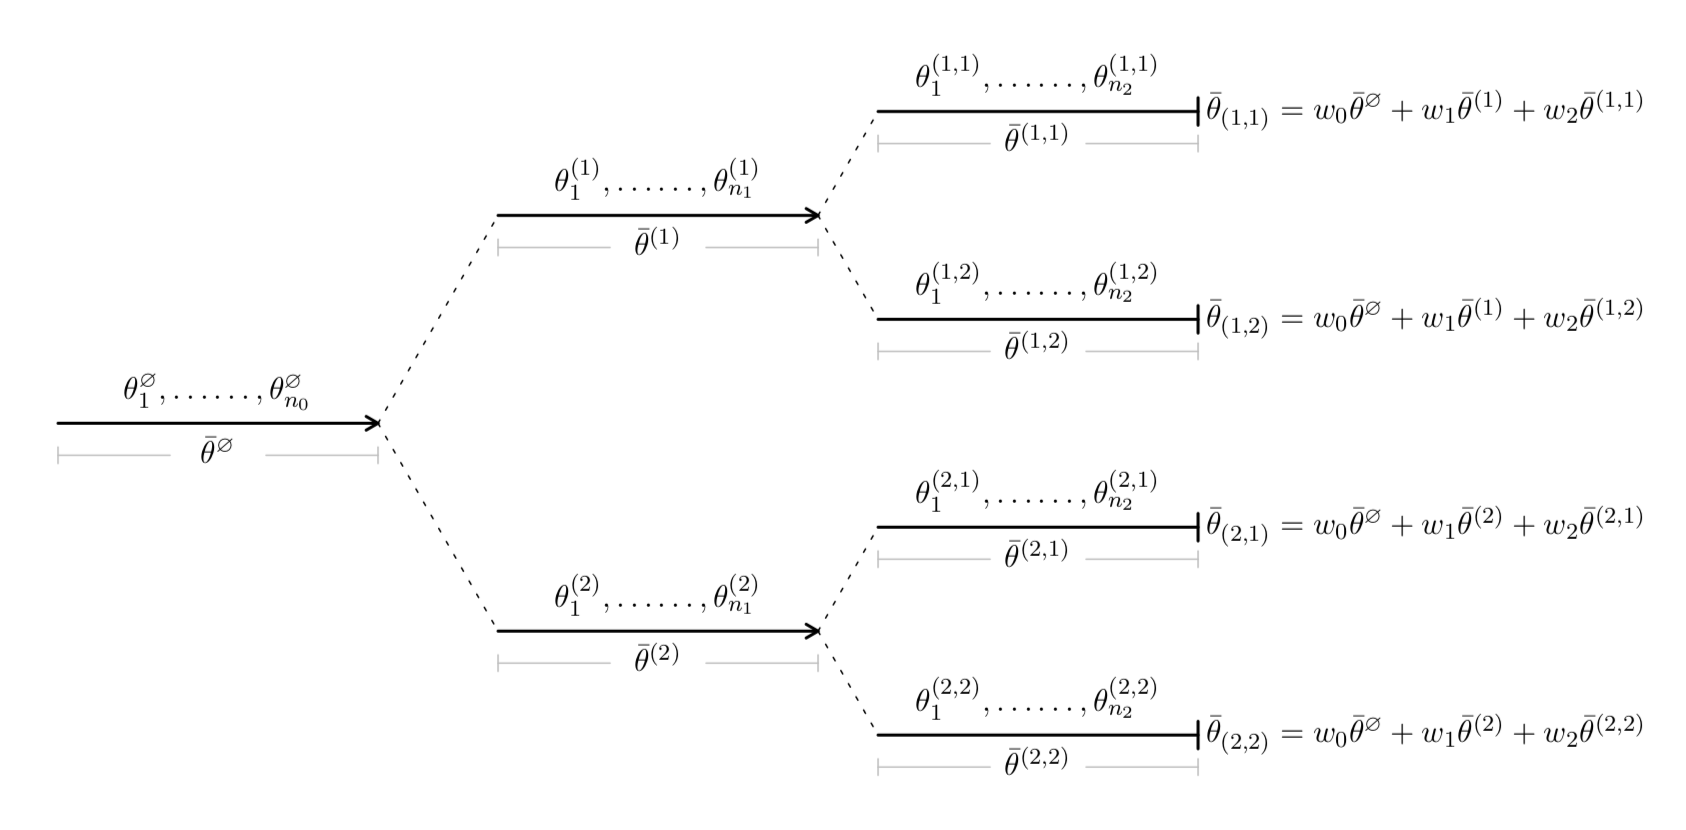
\includegraphics[width=0.5\textwidth]{HiGrad}
		\caption{HiGrad}
\end{figure}

If we have $T$ threads in total. Let
$$
\mu _ { x } ^ { * } = c^T\theta^*; \ \ 
\boldsymbol { \mu } _ { x } = c^T\begin{pmatrix} \bar\theta_1 \\ ... \\ \bar\theta_T\end{pmatrix} = \begin{pmatrix} \mu^1_x \\ ... \\ \mu^T_x\end{pmatrix}
$$

One can prove:
$$
\sqrt { N } \left( \boldsymbol { \mu } _ { x } - \mu _ { x } ^ { * } \mathbf { 1 } \right) \rightarrow \mathcal { N } \left( 0 , \sigma^2\Sigma\right)
$$

With $\Sigma$ can be computed by data. Asymptotically this is equivalent to the following linear regression with $\tilde { \boldsymbol { z } }$ be a whitened noise.
$$
\Sigma ^ { - \frac { 1 } { 2 } } \boldsymbol { \mu } _ { x } = \left( \Sigma ^ { - \frac { 1 } { 2 } } \mathbf { 1 } \right) \mu _ { x } ^ { * } + \tilde { \boldsymbol { z } }
$$

Thus we can easily obtain the least square estimator for $\mu _ { x } ^ { * } $:
$$
\overline { \mu } _ { x } : = \frac { 1 } { T } \sum _ { t = 1 }^{T} \mu _ { x } ^ { t }
$$

with standard deviation
$$
\mathrm { SE } _ { x } = \sqrt { \frac { \mathbf { 1 } ^ { \top } \Sigma \mathbf { 1 } \left( \boldsymbol { \mu } _ { x } ^ { \top } - \overline { \mu } _ { x } \mathbf { 1 } ^ { \top } \right) \Sigma ^ { - 1 } \left( \boldsymbol { \mu } _ { x } - \overline { \mu } _ { x } \mathbf { 1 } \right) } { T ^ { 2 } ( T - 1 ) } }
$$

Thus we can construct a confidence interval here
$$
\left[ \overline { \mu } _ { x } - t _ { T - 1,1 - \frac { \alpha } { 2 } } \mathrm { SE } _ { x } , \quad \overline { \mu } _ { x } + t _ { T - 1,1 - \frac { \alpha } { 2 } } \mathrm { SE } _ { x } \right]
$$



 % Don't be this informal in your notes!






